\documentclass[a4paper,fleqn]{cas-dc}

%\usepackage[authoryear,longnamesfirst]{natbib}
\usepackage[comma,numbers,square,sort&compress]{natbib}

\usepackage{graphicx} 
\usepackage{epstopdf}
\usepackage{bm}
\usepackage{amsmath}
\usepackage{amsthm}
\newtheorem{theorem}{Theorem}
\newtheorem{definition}{Definition}
\newtheorem{lemma}{Lemma}
\newtheorem{assumption}{Assumption}

\def\tsc#1{\csdef{#1}{\textsc{\lowercase{#1}}\xspace}}
\tsc{WGM}
\tsc{QE}


\begin{document}
	
	\let\WriteBookmarks\relax
	\def\floatpagepagefraction{1}
	\def\textpagefraction{.001}
	
% Short title
\shorttitle{Coordinated Path Following for Multiple Underactuated Surface Vessels}    

% Short author
\shortauthors{Yinsong Qu et al}  

% title
\title[mode = title]{Coordinated Path Following for Multiple Underactuated Surface Vessels with Error Constraints and Input Saturation}

\tnotemark[1]

\tnotetext[1]{This document is the results of the research project
	funded by the National Science Foundation.}

%--------------------1-----------------------
\author[]{Yuchao Wang}[type=editor,
style=chinese,
auid=000,bioid=1]
\fnmark[1] 

%\ead[url]{www.cvr.cc,www.tug.org.in}

\credit{Conceptualization of this study, Methodology, Software}

%------------------2-------------------------
\author[] {Yinsong Qu}[
orcid=0000-0001-7511-2910]
\cormark[1]
\fnmark[2] 
\ead{qu13298110549@163.com} 

\credit{Data curation, Writing - Original draft preparation}


\address[]{College of Intelligent Systems Science and Engineering, Harbin Engineering University, Harbin 150001, P.~R.~China}

%-------------------------------------------
\cortext[cor1]{Corresponding author} 

\fntext[fn1]{This is the first author footnote. 
	but is common to third author as well.}

\fntext[fn2]{Another author footnote, this is a very long footnote
	and it should be a really long footnote. But this footnote is not
	yet sufficiently long enough to make two lines of footnote text.}

\fntext[fn3]{K. Berry is the editor of \TeX Live.}

\begin{abstract}[S U M M A R Y]
In this paper, the coordinated path following control of multiple underactuated surface vessels with error constraints is studied. By combining tan-type barrier Lyapunov functions, this paper proposes a novel coordinated guidance law composed by desired surge speed and heading angle for each vehicle. By assigning the same number of parameterized paths to vehicles, the coordinated error variable is introduced by the graph theory, and then the desired update law for the each parameter of path is propsed to accomplish the coordination task. To track the desired guidance signal quickly and accuratly with high robustness, the radial neural-nerwork controller is developed for each vehicle by backstepping technique, in which, the neural network is used to estimate the unknown kinetic disturbances instantaneously. All closed-loop traking errors are proved to be uniform ultimately bounded by Lyapunov theory. In addition, the coordinated path following erros are bounded in the prescibed boundaries.
\end{abstract}
\begin{keywords}
	Coordinated path following \sep underactuated surface vessels \sep 
	error constraints \sep Input saturation \sep Neural network
\end{keywords}

\maketitle

\section{Introduction}
In the past two decades, the coordinated control of underactuated surface vessels (USVs) has attracted more and more attention due to its high efficiency in performing complicated tasks such as environmental monitoring and chart mapping. According to the different guidance signal, the coordinated control can be divided as path-guided coordinated control, trajectory-guided coordinated control and target-guided coordinated control. Compared to the another two methods, the path-guided coordinated control method can provide smoother guidance signals and trajectories. In this paper, we study the coordinated path following (CPF) control of USVs with error constraints.

There are many studies have been made for coordinated path following. In \cite{bib1}, the integral action is added into line-of-sight (LOS) guidance law to compensate for the adverse effects caused by currents, and the vessels achieve the formation task by assigning different velocities to each USV according to relative inter-vessel distance. The method proposed in \cite{bib1} is verified by CybershipII in \cite{bib2}. In \cite{bib3}, the cyber attack is modeled as a time-varying state-dependent variable. An adaptive term is incorporated into the coordinated guidance law to compensate the time-varying cyber attack. In \cite{bib4}, the event-triggering mechanism (ETM) is developed to reduce the communication cost among the USVs.  To estimate and cancel the unknown external disturbances, the extended state observer (ESO) is proposed in \cite{bib5}. In order to accelerate the convergence of errors, the finite-time CPF controllers based on fast terminal sliding mode control (FTSMC) technique are proposed in \cite{bib6}. Considering the unmeasurable velocities of USVs, the output-feedback control law is designed in \cite{bib7}. Above coordinated guidance laws above are based on LOS. Besides LOS, there also exist other guidance methods. In \cite{bib8}, the desired path is expressed in an implicit function, the coordinated guidance law is proposed by the sliding mode control (SMC) techinique. The guiding vector field (GVF) is proposed for CPF in \cite{bib9}, and is varified by unmmaned aerial vehicle (UAV) in \cite{bib10}.  Compared with GVF, LOS is able to provide smoother guidance signal and achieve global convergence of tracking errors. Therefore, we will use LOS to design the coordinated guidance law in this paper. 

Different from the above methods, the constraints of the path following errors will be considered in this paper. The tan-type barrier Lyapunov function (BLF) is introduced to design coordinated guidance law. In \cite{bib11}, the error-constrained LOS (ELOS) is proposed for single USV to realize the constraints of path following errors. In this paper, we will extended this method to CPF for multiple USVs. Different from \cite{bib12}, the unknown kinetic disturbances are considerd in this paper. The radial basis function neural network (RBFNN) is introduced to estimate the lumped kinetic disturbances. 

The main contributions of this paper are listed as follows:

1) The tan-type BLF are constructed to effectively guarantee the transient performance of each USV.

2) By assigning a parameterized path to each USV, the coordinated error variable is introduced by the graph theory, and then the desired update law for the each parameter is propsed to accomplish the coordination task.

3) It is proven that all errors of the closed-loop control system are uniform ultimately bounded (UUB) by using the proposed control method.

The rest of this paper is organized as follows. Section 2 formulates the CPF problem of multiple USVs. In Section 3, the coordinated control law is designed for CPF by Backstepping method. The stability analysis of the closed-loop system is given in Section 4. Simulation studies is conducted in Section 5. Section 6 concludes this paper.

\section{Problem Fomulation}
\subsection{Mathmatical Model}
The kinematics of $i$th USV are given as:

\begin{flalign}\label{kinematics}
&\	\left\{
	\begin{aligned}
		\dot{x}_i&=u_i\cos(\psi_i)-v_i\sin(\psi_i)\\
		\dot{y}_i&=u_i\sin(\psi_i)+v_i\cos(\psi_i)\\
		\dot{\psi}_i&=r_i\\
	\end{aligned}
	\right. &
\end{flalign}
where $x_i$ and $y_i$ and $\psi_i$ are north position, east position and heading angle of $i$th USV expressed in frame $\{\mathcal{I}\}$ (see Fig.~\ref{CPF}), $u_i$, $v_i$ and $r_i$ denote the surge, sway and yaw velocities of $i$th USV respectively.

The kinetics of $i$th USV are given as \cite{bib13}:

\begin{flalign}\label{kinetics}
	&\
	\left\{
	\begin{aligned}
		m_{11}\dot{u}_{i}-m_{22}v_{i}r_{i}+d_{11}u_{i}&=T_{li}+T_{ri}+\delta_{u}\\
		m_{22}\dot{v}_i+m_{11}u_iv_i+d_{22}v_{i}&=\delta_{v}\\
		m_{33}\dot{r}_i-(m_{11}-m_{22})u_iv_i+d_{33}r_i&=(T_{li}-T_{ri})d_p+\delta_r\\
	\end{aligned}
	\right.
	&
\end{flalign}
where $m_{ll}$, $l=1,2,3$ denote the inertial masses of $i$th USV, $d_{ll}$ denote the damping terms of $i$th USV respectively, $T_{li}$ and $T_{ri}$ are thrust generated by the left and right thrusters, $d_p$ is the lateral distance from the centerline of the USV to the centerline of each thruster, $\delta_u$, $\delta_v$ and $\delta_r$ are the unknown external disturbances.

In practice, the thrust $T_{li}$ and $T_{ri}$ are always bounded due to the physical limitations of the thrusters. The satuaration can be descriebd as:

\begin{flalign}
	&\
	T_{qi}=sat(T_{qi}^c)=\left\{
	\begin{aligned}
	 &T_{qi}^+,& T_{qi}^c> T_{qi}^+\\
     &T_{qi}^c,  &T_{qi}^-\ge T_{qi}^c \le T_{qi}^+ \\
	 &T_{qi}^-,& T_{qi}^c < T_{qi}^-
	\end{aligned}
	\right.
	, q = l,r
	&
\end{flalign}
where $T_{qi}^c$ denote the thrust commands generated by controller , $T_{qi}^+$ and $T_{qi}^-$ denote the maimum and minimum thrust of thrusters. To overcome the sharp corners, the saturation nonlinearity is modeled by a smooth function with the form as

\begin{flalign}
	&\
	f(T_{qi}) = \left\{
	\begin{aligned}
			&T_{qi}^{+}\tanh\left(\frac{T_{qi}}{T_{qi}^+}\right), T_{qi}\ge 0\\
			&T_{qi}^{-}\tanh\left(\frac{T_{qi}}{T_{qi}^{-}}\right), T_{qi}\leq 0
	\end{aligned}
	\right.
	, q = l, r
	&
\end{flalign}

Let $\varrho_{qi}=T_{qi}-f(T_{qi})$ be the approximated error, and the $\varrho_{qi}^c=T_{qi}^c-f(T_{qi})$ be the saturated error. To facilitate control design, the kinetics are rewritten as

\begin{flalign}\label{kinetics 2}
	&\ 
	\dot{\bm{\xi}}_i=\bm{F}_{\xi i}+\bm{G}\bm{T}_i^c-G\bm{\varrho}_i^c
	&
\end{flalign}
where $\bm{\xi}_i=[u_i,r_i]^{\rm T}$, $\bm{T}_i=\left[T_{li},T_{ri}\right]^T$, $\bm{F}_{\xi i}=\left[f_{ui},f_{ri}\right]^T$, $\varrho_i^c=\left[\varrho_{li}^c,\varrho_{ri}^c\right]$, $\bm{F}_{\xi i}$ and $\bm{G}$ are given as\\
\begin{flalign}
	&\
	\bm{F}_{\xi i}=
	\begin{bmatrix}
		\frac{m_{22}v_ir_i}{m_{11}}-\frac{d_{11}u_i}{m_{11}}+\frac{\varrho_{li}+\varrho_{ri}}{m_{11}}\\
		\frac{(m_{11}-m_{22})u_iv_i}{m_{33}}-\frac{d_{33}r_i}{m_{33}}-\frac{d_p(\varrho_{ri}-\varrho_{li})}{m_{33}}
	\end{bmatrix},
	\bm{G}=
	\begin{bmatrix}
		\frac{1}{m_{11}} && \frac{1}{m_{11}}\\
		\frac{d_p}{m_{33}} && -\frac{d_p}{m_{33}}
	\end{bmatrix}
	&
\end{flalign}

\begin{figure}[!htb]
	\centering
	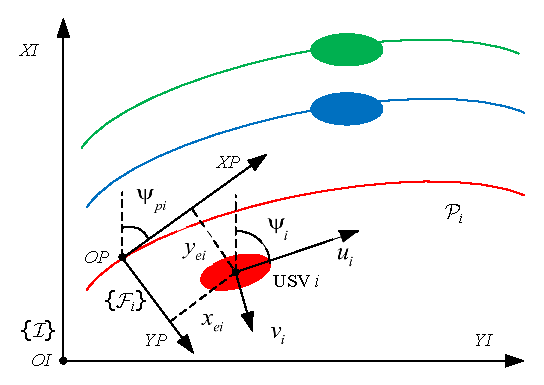
\includegraphics[width=\hsize]{CPF.eps}
	\caption{The framework of coordinated path following. }
	\label{CPF}
\end{figure}

\subsection{Control Objective}

Assuming there are $N$ USVs, we will assign $N$ parameterized paths to these USVs. Then, the CPF control objective can be divided into two parts, for the first part, the $i$th USV is required to follow the $i$th path, which is named as heading control, for the second part, the $i$th USV is required to hold desired distance to another USV, which is named as speed control. In this section, we will give the control objective of coordinated path following.

The path following errors can be represented by the positions of $i$th USV in the frame $\mathcal{F}_i$ denoted by $x_{ei}$ and $y_{ei}$, which are calculated as:

\begin{flalign}\label{path following error}
	&\
	\begin{bmatrix}
		x_{ei} \\ y_{ei}
	\end{bmatrix}=
	\begin{bmatrix}
		\cos(\psi_{pi}) & \sin(\psi_{pi})\\
		-\sin(\psi_{pi}) & \cos(\psi_{pi})\\
	\end{bmatrix}
	\begin{bmatrix}
		x_i-x_{pi}(\theta_i) \\ y_i-y_{pi}(\theta_i)
	\end{bmatrix}
	&
\end{flalign}
where $\psi_{pi}$ is the angle of the $i$th path $\mathcal{P}_i$ at point $P$ with respect to the inertial XI-axis (see Fig.~\ref{CPF}), $\psi_{pi}=\arctan2(y^{'}_{pi},x^{'}_{pi})$, $\theta_i$ is the parameter of $i$th path. Combining with ($\ref{kinematics}$) and (\ref{path following error}), the derivatives of $x_{ei}$ and $y_{ei}$ are calculated as:

\begin{flalign}
	&\
	\left\{
	\begin{aligned}
		\dot{x}_{ei}&=u_i\cos(\psi_{ei})-v_i\sin(\psi_{ei})+k_{ci}u_{pi}y_{ei}-u_{pi}\\
		\dot{y}_{ei}&=u_i\sin(\psi_{ei})+v_i\cos(\psi_{ei})-k_{ci}u_{pi}x_{ei}\\
	\end{aligned}
	\right.
	&
\end{flalign}
where $u_{pi}=u^*_{pi}\dot{\theta}_i$, $u^*_{pi}=\sqrt{x^{'2}_{pi}+y^{'2}_{pi}}$.

Considering the virtual leader $\mathcal{V}_0$ and $N$ agents, we assign a parameter $\theta_0$ to $\mathcal{V}_0$. Then, the coordinated errors can be defined as:

\begin{flalign}\label{coordinated error}
	&\
	e_{\theta i}=\sum^N_{j=1}a_{ij}(\theta_i-\theta_j-d_{\theta ij})+b_i(\theta_i-\theta_0-d_{\theta i0})
	&
\end{flalign}

The derivative of $e_{\theta i}$ is

\begin{flalign}
	&\
	\dot{e}_{\theta i}=\sum_{j\in Ni}a_{ij}(\frac{u_{pi}}{u^*_{pi}}-\frac{u_{pj}}{u^*_{pj}})+b_i(\frac{u_{pi}}{u^*_{pi}}-\frac{u_{p0}}{u^*_{p0}})
	&
\end{flalign}

The path following errors and coordinated errors are expressed in (\ref{path following error}) and (\ref{coordinated error}). In the following, we given the control objectives of coordinated path following.

\emph{O1}) Heading control: The $i$th USV is required to follow the given path $P_i$ with the desired heading angle $\psi_{ci}$, and the path following errors $x_{ei}$ and $y_{ei}$ will be constrained in the prescibed boundaries for the specified initial condition, i.e., $\lim_{t\to \infty}\left|x_{ei}\right|< \sigma_{xi}$ and $\lim_{t\to \infty}\left|y_{ei}\right|< \sigma_{yi}$ for the initial condition $\lim_{t\to \infty}\left|x_{ei}(0)\right|< \sigma_{xi}(0)$ and $\lim_{t\to \infty}\left|y_{ei}(0)\right|< \sigma_{yi}(0)$, where $\sigma_{xi}$ and $\sigma_{yi}$ are prescribed boundaries.

\emph{O2}) speed control: All the USVs will achieve the desired formation by regulating surge speed, i.e., the desired speed $u_{pi}$ will be assigned to each USV such that the following relations hold, $\lim_{t\to \infty}\left|e_{\theta i}\right|<d_1$, and there is $\lim_{t\to \infty}\left|u_{i}-u_{pi}\right|<d_2$, where $d_1$ and $d_2$ are small positive constants. 

\subsection{Graph Theory}

Consider a directed graph $\mathcal{G}=\{\mathcal{N},\varepsilon\}$, where $\mathcal{N}=\{\mathcal{V}_1,\mathcal{V}_2,...,\mathcal{V}_N\}$ denote the set of $N$ nodes and $\varepsilon=\{(\mathcal{V}_i,\mathcal{V}_j)\in \mathcal{N}\times \mathcal{N}\}$ is the edge set. The node $\mathcal{V}_i$ can get the information from node $\mathcal{V}_j$ if $(\mathcal{V}_i,\mathcal{V}_j)\in \varepsilon$. The communication topology between $\mathcal{V}_i$ and $\mathcal{V}_j$ is represented by the adjacency matrix $\bm{\mathcal{A}}=[a_{ij}]\in \mathbb{R}^{n\times n}$, where $a_{ij}=1$ if $(\mathcal{V}_i,\mathcal{V}_j)\in \varepsilon$ and $i\neq j$, $a_{ij}=0$ otherwise. Let $\bm{\mathcal{D}}={\rm diag}\{d_1,d_2,...,d_N\}$ where $d_i=\sum^N_{j=1}a_{ij},i=1,2,...,N$. The Laplacian matrix of $\mathcal{G}$ is defined as $\bm{\mathcal{L}}=\bm{\mathcal{D}}-\bm{\mathcal{A}}$. The communication between node $\mathcal{V}_i$ and the virtual leader $\mathcal{V}_0$ is represented by the leader adjacency matrix $\bm{\mathcal{B}}={\rm diag}\{b_1,b_2,...,b_N\}\in \mathbb{R}^{n\times n}$, where $b_i=1$ if node $\mathcal{V}_i$ can obtain information from virtual leader, $b_i=0$ otherwise. 

\begin{definition}
	Spnning tree: There is a root node for the graph $\mathcal{G}$ such that there always exist a directed path from the root vertex to another node of $\mathcal{G}$.  
\end{definition}

\begin{assumption}\label{assumption}
	The graph $\mathcal{G}$ has a spanning tree with the root node $\mathcal{V}_0$.
\end{assumption}

\begin{lemma}\label{lemma}
	Let $\bm{\mathcal{H}}=\bm{\mathcal{L}}+\bm{\mathcal{B}}$. All the eigenvalues of $\bm{\mathcal{H}}$ have positive real parts if and only if Assumption \ref{assumption} hold. In addition, there exists $\bm{Q}=\bm{Z}\bm{\mathcal{H}}+\bm{\mathcal{H}}^{\rm T}\bm{Z}$, where $\bm{Q}=[q_1,q_2,...,q_N]^{\rm T}=\bm{\mathcal{H}}^{-1}\bm{1}_n$, $\bm{Z}={\rm diag}\{1/q_i\}$. {\rm (see \cite{bib14,bib15})}
\end{lemma} 

\section{Coordinated guidance law}
In the section, we will design the coordinated guidance law and neural-network (NN) controller for each USV by backstepping method and graph theory.

\subsection{Estimations of velocities}
To get the estimations of linear velocities, the error dynamics can be rewritten as follows

\begin{flalign}
	&\
	\left\{
	\begin{aligned}
		&\dot{x}_{ei}=\chi_{xi}+k_{ci}u_{pi}y_{ei}-u_{pi}\\
		&\dot{y}_{ei}=\chi_{yi}-k_{ci}u_{pi}x_{ei}
	\end{aligned}
	\right.
	&
\end{flalign}
where $\chi_{xi}=u_i\cos(\psi_{ei})-v_i\sin(\psi_{ei})$ and $\chi_{yi}=u_i\sin(\psi_{ei})+v_i\cos(\psi_{ei})$. Then the two ESOs can be designed as

\begin{flalign}
	&\
	\left\{
	\begin{aligned}
	\dot{\hat{x}}_{ei}=&\hat{\chi}_{xi}+k_{ci}u_{pi}y_{ei}-u_{pi}+\\
	&k_{ox1i}fal(r_{oxi}(x_{ei}-\hat{x}_{ei}),\iota_{xi},d_{xi})\\
	\dot{\hat{\chi}}_{xi} =& r_{oxi}k_{ox2i}fal(r_{oxi}(x_{ei}-\hat{x}_{ei}),\iota_{xi},d_{xi})
	\end{aligned}
	\right.
	&
\end{flalign}

\begin{flalign}
	&\
	\left\{
	\begin{aligned}
		\dot{\hat{y}}_{ei}=&\hat{\chi}_{yi}-k_{ci}u_{pi}y_{ei}+\\
		&k_{oy1i}fal(r_{oyi}(y_{ei}-\hat{y}_{ei}),\iota_{yi},d_{yi})\\
		\dot{\hat{\chi}}_{yi} =& r_{oyi}k_{oy2i}fal(r_{oyi}(y_{ei}-\hat{y}_{ei}),\iota_{yi},d_{yi})
	\end{aligned}
	\right.
	&
\end{flalign}
where $fal(*,\iota,d)$ is defined as

\begin{flalign}
	&\
	fal(*,\iota,d)= 
	\left\{
	\begin{aligned}
		&\frac{*}{d}, &|*|\le d\\
		&|\iota|^\iota sign(x), &|*|> d
	\end{aligned}
	\right.
	&
\end{flalign}

Define the estimated errors as $\tilde{x}_{ei}=x_{ei}-\hat{x}_{ei}$, $\tilde{y}_{ei}=y_{ei}-\hat{y}_{ei}$, $\tilde{\chi}_{xi}=\chi_{xi}-\hat{\chi}_{xi}$, $\tilde{\chi}_{yi}=\chi_{yi}-\hat{\chi}_{yi}$. Then, there is

\begin{flalign}
	&\
	\left\{
	\begin{aligned}
		\dot{\tilde{x}}_{ei}=&\tilde{\chi}_{xi}-k_{ox1i}fal(r_{oxi}(\tilde{x}_{ei}),\iota_{xi},d_{xi})\\
		\dot{\tilde{\chi}}_{xi} =& -r_{oxi}k_{ox2i}fal(r_{oxi}(\tilde{x}_{ei}),\iota_{xi},d_{xi})+\dot{\chi}_{xi}
	\end{aligned}
	\right.
	&
\end{flalign}

\begin{flalign}
	&\
	\left\{
	\begin{aligned}
		\dot{\tilde{y}}_{ei}=&\tilde{\chi}_{yi}-k_{ci}u_{pi}y_{ei}-\\
		&k_{oy1i}fal(r_{oyi}(\tilde{y}_{ei}),\iota_{yi},d_{yi})\\
		\dot{\tilde{\chi}}_{yi} =& r_{oyi}k_{oy2i}fal(r_{oyi}(\tilde{y}_{ei}),\iota_{yi},d_{yi})+\dot{\chi}_{yi}
	\end{aligned}
	\right.
	&
\end{flalign}

Due to the relation between $\chi_{xi}$, $\chi_{yi}$ and $u_i$, $v_i$, we can get the estimations of velocities as

 \begin{flalign}
 	&\
 	\left\{
 	\begin{aligned}
 		\hat{u}_i=&\hat{\chi}_{xi}\cos(\psi_{ei})+\hat{\chi}_{yi}\sin(\psi_{ei})\\
 		\hat{v}_i=&\hat{\chi}_{xi}cos(\psi_{ei})-\hat{\chi}_{yi}\sin(\psi_{ei})
 	\end{aligned}
 	\right.
 	&
 \end{flalign}
	
Define the estimated errors as $e_{ui}=u_i-\hat{u}_i$ and $e_{vi}=v_i-\hat{v}_i$. There is

 \begin{flalign}
	&\
	\left\{
	\begin{aligned}
		\tilde{u}_i=&\tilde{\chi}_{xi}\cos(\psi_{ei})+\tilde{\chi}_{yi}\sin(\psi_{ei})\\
		\tilde{v}_i=&\tilde{\chi}_{xi}cos(\psi_{ei})-\tilde{\chi}_{yi}\sin(\psi_{ei})
	\end{aligned}
	\right.
	&
\end{flalign}

\subsection{Guidance law design}
Define traking errors as $\tilde{u}_i=u_i-u_{ci}-\lambda_{ui}$, $\tilde{\psi}_i=\psi_i-\psi_{ci}$, $\tilde{r}_i=r_i-r_{ci}-\lambda_{ri}$, then, the error dynamics of (\ref{path following error}) can be rewritten as:

\begin{flalign}\label{path following error dynamics 1}
	&\
	\left\{
	\begin{aligned}
		\dot{x}_{ei}=&u_{ci}-2\hat{u}_i\sin^2(\frac{\psi_{ei}}{2})-\hat{v}_i\sin(\psi_{ei})+\\&k_{ci}u_{pi}y_{ei}-u_{pi}+f_{xi}+\tilde{u}_i\\
		\dot{y}_{ei}=&\hat{U}_{ci}\sin(\psi_{ci}-\psi_{pi}+\hat{\beta}_{ci})-k_{ci}u_{pi}x_{ei}+\\&f_{yi}+\tilde{u}_i\sin(\psi_{e})+\hat{U}_{ci}\omega_i\tilde{\psi}_i
	\end{aligned}
	\right.
	&
\end{flalign}
where $\omega_i=\frac{\cos(\psi_{ci}-\psi_{pi}+\beta_i)\sin(\tilde{\psi}_i)+\sin(\psi_{ci}-\psi_{pi}+\beta_i)(\cos(\tilde{\psi}_i)-1)}{\tilde{\psi}_i}$, $\hat{U}_{ci}=\sqrt{u^2_{ci}+\hat{v}^2_{i}}$, and $\hat{\beta}_{ci}=\arctan({\frac{\hat{v}_i}{u_{ci}}})$, $f_{xi}=\lambda_{ui}+e_{ui}-2e_{ui}\sin^2(\psi_{ei}/2)-e_{vi}\sin(\psi_{ei})$ and $f_{yi}=(\lambda_{ui}+e_{ui})\sin(\psi_{ei})+e_{vi}\cos(\psi_{ei})$.

Althogh the nonlinear functions $f_{xi}$ and $f_{yi}$ are unknown, they satisfy the following condition

 \begin{flalign}\label{eq20}
 	&\
 	f_{x,i} = \Theta^T\Omega_{xi}(x_e,y_e), f_{y,i} = \Theta^T\Omega_{yi}(x_e,y_e)
 	&
 \end{flalign}
where $\Omega_{xi}$ and $\Omega_{yi}$ are smooth functions, and $\Theta$ is uncertain parameter which is bounded. To compensate the unknown functions $f_{xi}$ and $f_{yi}$, 
we introduce the adaptive parameter $\hat{\Theta}$, which is the estimated value of $\Theta$. The estimated errors is defined as $\tilde{\Theta}=\hat{\Theta}-\Theta$. To realize the constraints on the path following errors, The first Lypunov function is construct as the tan-type BLF:

\begin{flalign}\label{V1}
	&\
	V_{1i}=\frac{\sigma^2_{xi}}{\pi}\tan(\frac{\pi x_{ei}^2}{2\sigma^2_{xi}})+\frac{\sigma^2_{yi}}{\pi}\tan(\frac{\pi y_{ei}^2}{2\sigma^2_{yi}})+\frac{1}{2}\tilde{\Theta}^T\Gamma_{\Theta}\tilde{\Theta}
	&
\end{flalign}
where $\sigma_{xi}$ and $\sigma_{yi}$ are the prescribed boundaries. Assuming the parameters $\Theta_{xi}$ and $\Theta_{yi}$ are constant values, the derivative of $V_{1i}$ can be calculated as:

\begin{flalign}\label{V1dot0}
	&\
	\begin{aligned}
		\dot{V}_{1i}&=\frac{2\sigma_{xi}\dot{\sigma}_{xi}}{\pi}\tan(\frac{\pi x_{ei}}{2\sigma^2_{xi}})+x_{ei}\dot{x}_{ei}\sec^2(\frac{\pi x_{ei}}{2\sigma^2_{xi}})-\\
		&\frac{\dot{\sigma}_{xi}}{\sigma_{xi}}x^2_{ei}\sec^2(\frac{\pi x_{ei}}{2\sigma^2_{xi}})+\frac{2\sigma_{yi}\dot{\sigma}_{yi}}{\pi}\tan(\frac{\pi x_{ei}}{2\sigma^2_{xi}})+\\
		&y_{ei}\dot{y}_{ei}\sec^2(\frac{\pi y_{ei}}{2\sigma^2_{yi}})-\frac{\dot{\sigma}_{yi}}{\sigma_{yi}}y^2_{ei}\sec^2(\frac{\pi y_{ei}}{2\sigma^2_{yi}})+\tilde{\Theta}^T\Gamma_{\Theta}\dot{\hat{\Theta}}
	\end{aligned}
	&
\end{flalign}

Combining with (\ref{path following error dynamics 1}) and (\ref{V1dot0}), the desired heading angle and surge speed are given as:

\begin{flalign}\label{guidance law 1}
	&\
	\left\{
	\begin{aligned}
		u_{ci}=&2\hat{u}_i\sin^2(\frac{\psi_{ei}}{2})+\hat{v}_i\sin(\frac{\psi_{ei}}{2})+\alpha_i-\rho_{xi}\\
		\psi_{ci}=&\psi_{pi}-\hat{\beta}_{ci}-\arctan(\frac{\rho_{yi}}{\Delta_i})\\
		\dot{\hat{\Theta}}=&\Gamma_{\Theta}(w_{xi}x_{ei}\sec^2(\frac{\pi x_{ei}^2}{2\sigma_{xi}^2})+w_{yi}y_{ei}\sec^2(\frac{\pi y_{ei}^2}{2\sigma_{yi}^2}))
	\end{aligned}
	\right.
	&
\end{flalign}
where $\Delta_i>0$ denotes the look-ahead distance, $w_{yi}=\frac{\hat{U}_{ci}}{\sqrt{\rho_{yi}^2+\Delta_i^2}}$, $w_{xi}$ is chosen later, and there is

\begin{flalign}
	&\
	\left\{
	\begin{aligned}
		\rho_{xi}=&\frac{k_{x1i}\sigma^2_{xi}}{\pi x_{ei}}\sin(\frac{\pi x^2_{ei}}{2\sigma^2_{xi}})\cos(\frac{\pi x^2_{ei}}{2\sigma^2_{xi}})+k_{x2i}x_{ei}-\hat{\Theta}w_{xi}\\
		\rho_{yi}=&\frac{k_{y1i}\sigma^2_{yi}}{\pi y_{ei}}\sin(\frac{\pi y^2_{ei}}{2\sigma^2_{yi}})\cos(\frac{\pi y^2_{ei}}{2\sigma^2_{yi}})+k_{y2i}y_{ei}-\hat{\Theta}\\
		\alpha_i=&u^*_{pi}\left(1-k_{ci}y_{ei}\left(1-\cos^2(\frac{\pi x^2_{ei}}{2\sigma^2_{xi}})\sec^2(\frac{\pi y^2_{ei}}{2\sigma^2_{yi}})\right)\right)\\
	\end{aligned}
	\right.
	&
\end{flalign}
where $k_{x1i}$, $k_{x2i}$, $k_{y1i}$ and $k_{y2i}$ are positive parameters which will be discussed in Section 4.

Combining with (\ref{path following error dynamics 1}) and (\ref{guidance law 1}), (\ref{V1dot}) can be further calculated as

\begin{flalign}\label{V1dot}
	&\
	\begin{aligned}
		\dot{V}_{1i}&=-\frac{k_{x1i}\sigma^2_{xi}}{\pi}\tan(\frac{\pi x^2_{ei}}{2\sigma^2_{xi}})-k_{x2i}x^2_{ei}\sec^2(\frac{\pi x^2_{ei}}{2\sigma^2_{xi}})-\\
		&\frac{U_ik_{y1i}\sigma^2_{yi}}{\pi\sqrt{\Delta^2_i+\rho_{yi}}}\tan(\frac{\pi y^2_{ei}}{2\sigma^2_{yi}})-\frac{\dot{\sigma}_{xi}}{\sigma_{xi}}x^2_{ei}\sec^2(\frac{\pi x^2_{ei}}{2\sigma^2_{xi}})-\\
		&\frac{U_ik_{y2i}y^2_{ei}}{\sqrt{\Delta^2_i+\rho^2_{yi}}}\sec^2(\frac{\pi y^2_{ei}}{2\sigma^2_{yi}})+\tilde{u}_ix_{ei}\sec^2(\frac{\pi x^2_{ei}}{2\sigma^2_{xi}})+\\
		&\tilde{u}_i\sin(\psi_{ei})\sec^2(\frac{\pi y^2_{ei}}{2\sigma^2_{yi}})+\frac{2\sigma_{xi}\dot{\sigma}_{xi}}{\pi}\tan(\frac{\pi x_{ei}}{2\sigma^2_{xi}})+\\
		&U_i\omega_i\tilde{\psi}_iy_{ei}\sec^2(\frac{\pi y^2_{ei}}{2\sigma^2_{yi}})+\frac{2\sigma_{yi}\dot{\sigma}_{yi}}{\pi}\tan(\frac{\pi y_{ei}}{2\sigma^2_{yi}})-\\
		&\frac{\dot{\sigma}_{yi}}{\sigma_{yi}}y^2_{ei}\sec^2(\frac{\pi y^2_{ei}}{2\sigma^2_{yi}})
	\end{aligned}
	&
\end{flalign}

The second Lyapunov function is chosen as

\begin{flalign} \label{V2}
	&\
	V_{2i}=0.5\tilde{\psi}^2_i
	&
\end{flalign}

The derivative of $V_2$ is 

\begin{flalign} \label{V2dot}
	&\
	\dot{V}_{2i}=\tilde{\psi}_i(r_{ci}+\tilde{r}_i-\dot{\psi}_{ci})
	&
\end{flalign}

The desired yaw velocity is designed as

\begin{flalign} \label{desired yaw velocity}
	&\
	r_{ci}=\dot{\psi}_{ci}-k_{ri}\tilde{\psi}_i-U_i\rho_iy_{ei}\sec^2(\frac{\pi y^2_{ei}}{2\sigma^2_{yi}})
	&
\end{flalign}

Substituting (\ref{desired yaw velocity}) into (\ref{V2dot}), we can get

\begin{flalign} \label{V2dot}
	&\
	\dot{V}_{2i}=-k_{ri}\tilde{\psi}^2_i-U_i\rho_i\tilde{\psi}_iy_{ei}\sec^2(\frac{\pi y^2_{ei}}{2\sigma^2_{yi}})
	&
\end{flalign}

\section{Neuro-adaptive Controller}
Let $\bm{\xi}_i=[u_i,r_i]^{\rm T}$, $\bm{\xi}_{ci}=[u_{ci},r_{ci}]^{\rm T}$. The tracking error can be rewritten as $\tilde{\bm{\xi}}_i=\bm{\xi}-\bm{\xi}_{ci}-\bm{\lambda}$, where $\lambda=[\lambda_{ui},\lambda_{ri}]^T$. 
To overcome the input saturation, the first order auxiliary system is given as

\begin{flalign}
	&\
	\dot{\bm{\lambda}}_i = -\Lambda\bm{\lambda}-\bm{G}\varrho^c_i
	&
\end{flalign}

The derivative of $\tilde{\bm{\xi}}_i$ is

\begin{flalign}
	&\
	\dot{\tilde{\bm{\xi}}}_i=\bm{F}_{\xi i}+\bm{G}\bm{T}_i+\Lambda\lambda-\dot{\bm{\xi}}_{ci}
	&
\end{flalign}

Since the nonlinear term $\bm{F}_{\xi i}$ is unknown, the neural network is used to approximate it as follows

\begin{flalign}
	&\
	\bm{F}_{\xi i}=\bm{W}^{\rm T}_i\bm{\Phi}_i(\bm{X}_i)+\bm{\zeta}_i(\bm{X}_i)
	&
\end{flalign}
where $\bm{W}_i$ is the desired weight matrix of neural network, which is unknown but bounded, $\bm{X}_i$ is the input vector of NN, $\bm{\Phi}_i(\bm{X}_i)$ is the radial basis function, and $\bm{\zeta}_i(\bm{X}_i)$ is the approximate error.  

The third Lyapunov function is chosen as

\begin{flalign}
	&\
	V_{3i}=0.5\tilde{\bm{\xi}}^{\rm T}_i\tilde{\bm{\xi}}_i+0.5{\rm tr}(\tilde{\bm{W}}^{\rm T}_i\Gamma^{-1}_{Wi}\tilde{\bm{W}}_i)+0.5\bm{\lambda}^T
	\bm{\lambda}
	&
\end{flalign}

Then, we can get the propotinal type feedback control law as

\begin{flalign}\label{control law}
	&\
	\bm{T}_i=\bm{G}^{-1}(\dot{\bm{\xi}_{ci}}-\hat{\bm{W}}^{\rm T}\bm{\Phi}_i(\bm{X}_i)-\bm{K}_{\xi i}\tilde{\bm{\xi}}_i+\bm{\rho}_{\xi i}-\Lambda\lambda)
	&
\end{flalign}
where $\hat{\bm{W}}_i$ is estimated value of $\bm{W}_i$, $\bm{\rho}_{\xi i}=[x_{ei}\sec^2(\frac{\pi x^2_{ei}}{2\sigma^2_{xi}})+y_{ei}\sin(\psi_{ei})\sec^2(\frac{\pi y^2_{ei}}{2\sigma^2_{yi}}),\tilde{\psi}_i]^{\rm T}$.

The update law is designed as

\begin{flalign}\label{update law}
	&\
	\dot{\hat{\bm{W}}}_i=\Gamma_{Wi}(\bm{\Phi}_i(\bm{X}_i)\tilde{\bm{\xi}}^{\rm T}_i-\bm{K}_{Wi}\hat{\bm{W}}_i)
	&
\end{flalign}

Combined with (\ref{control law}) and (\ref{update law}), the derivative of $V_3$ can be calculated as

\begin{flalign}\label{V3dot}
	&\
	\dot{V}_{3i}=-\tilde{\bm{\xi}}^{\rm T}_i\bm{K}_{\xi i}\tilde{\bm{\xi}}_i+k_{Wi}{\rm tr}(\tilde{\bm{W}}^{\rm T}_i\hat{\bm{W}}_i)+\tilde{\bm{\xi}}^{\rm T}_i\bm{\rho}_{\xi i}-\bm{\lambda}^T\Lambda\bm{\lambda}-\bm{\lambda}^T\bm{G}\bm{\varrho}_i^c
	&
\end{flalign}

The control law for path following is completed here. To realize the formation task, the coordinated guidance law is designed as follows.

Step 4. Let $\bm{E}_\theta=\left[e_{\theta 1},e_{\theta 2}...,e_{\theta n}\right]^{\rm T}$, there is $\bm{E}_\theta=\bm{\mathcal{H}}(\bm{\theta}-\theta_0\bm{1}_n)$. The derivative of $\bm{E}_\theta$ is

\begin{flalign}\label{coordinated error dynamics}
	&\
	\dot{\bm{E}}_\theta=\bm{\mathcal{H}}
	\begin{bmatrix}
		\frac{u_{p1}}{u^*_{p1}}-\frac{u_{p0}}{u^*_{p0}}\\
		...\\
		\frac{u_{pn}}{u^*_{pn}}-\frac{u_{p0}}{u^*_{p0}}\\
	\end{bmatrix}
	&\
\end{flalign}

The fourth Lyapunov function can be chosen as

\begin{flalign}
	&\
	V_4=0.5\bm{E}^{\rm T}_\theta \bm{Q} \bm{E}_\theta
	&\
\end{flalign}

The coordinated guidance law is designed as

\begin{flalign}\label{coordinated guidance law}
	&\
	u_{pi}=u^{*}_{pi}(\frac{u_0}{u^*_{p0}}-k_{\theta i}e_{\theta i})
	&\
\end{flalign}

Then, the update law of the parameter of path $i$ is $\dot{\theta}_i=\frac{u_{pi}}{u^*_{pi}}$.

Combined with (\ref{coordinated guidance law}) and (\ref{coordinated error dynamics}), the derivative of $V_4$ is calculated as

\begin{flalign}\label{V4dot}
	&\
	\dot{V}_4=0.5\bm{E}^{\rm T}_\theta(\bm{K}^{\rm T}_\theta \bm{\mathcal{H}}^{\rm T}\bm{Q}+\bm{Q}\bm{\mathcal{H}}\bm{K}_\theta)\bm{E}_\theta
	&
\end{flalign}

The coordinated control law for CPF is completed here. The block diagram of the control system for CPF is illustrated in Fig.~\ref{CPFCS}.

\begin{figure*}[!htb]
	\centering
	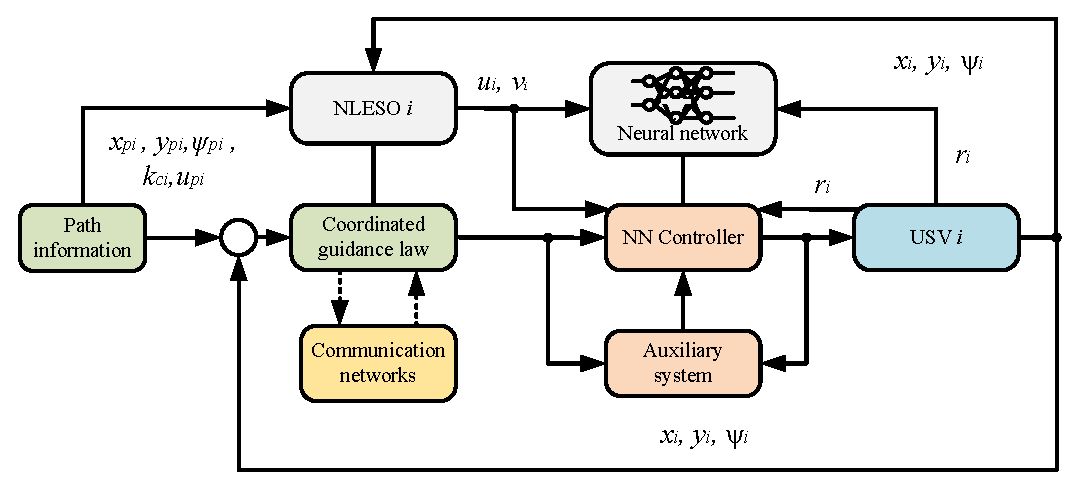
\includegraphics[width=12cm]{CPFCS.eps}
	\caption{Block diagram of Coordinited path following control system.}
	\label{CPFCS}
\end{figure*}

\section{Stability Analysis}

\begin{theorem}
	The path following errors $x_{ei}$, $y_{ei}$, and tracking errors $\tilde{u}_i$, $\tilde{\psi}_i$, $\tilde{r}_i$ will be UUB, if there exist parameters $k_{x1i}$, $k_{x2i}$, $k_{y1i}$, and $k_{y2i}$ such that the equalities given in (\ref{condition}) hold. In addition, the path following errors will be constrained in the prescribed boundaries $\sigma_{xi}$ and $\sigma_{yi}$, i.e., $\left|x_{ei}\right|\leq \sigma_{xi}$ and $\left|y_{ei}\right|\leq \sigma_{yi}$,  for the given initial value $\left|x_{ei}(0)\right|\leq \sigma_{xi}(0)$ and $\left|y_{ei}(0)\right|\leq \sigma_{yi}(0)$. \end{theorem}

\begin{flalign}\label{condition}
	&\
	\left\{
	\begin{aligned}
		k_{x2i}=&\sqrt{\frac{\dot{\sigma}_{xi}}{\sigma_{xi}^2}+k_{x0i}}\\
		k_{y2i}=&\frac{\dot{\sigma}_{yi}\sqrt{\Delta_i(\sigma^2_{ui}-\dot{\sigma}^2_{yi}y^2_{ei})+k^2_{y0i}\sigma^2_{ui}}+\dot{\sigma}^2_{yi}k_{y0i}y_{ei}}{\sigma^2_{ui}-\dot{\sigma}^2_{yi}}\\
	\end{aligned}
	\right.
	&
\end{flalign} 
where $\sigma^2_{ui}=\sigma^2_{yi}U^2_{ci}$, $k_{y0i}=\frac{k_{y1i}\sigma_{yi}^2}{\pi y_{ei}}\sin(\frac{\pi y_{ei}^2}{2\sigma_{yi}^2})\cos(\frac{\pi y_{ei}^2}{2\sigma_{yi}^2})$.

\begin{proof} 
	Construct the Lyapunov function as
	
	\begin{flalign}\label{V}
		&\
		V=V_4+\sum^3_{i=1}V_{1i}+V_{2i}+V_{3i}
		&
	\end{flalign}
	
	Under the condition (\ref{condition}), there are 
	
	\begin{flalign}\label{relation}
		&\
		\left\{
		\begin{aligned}
			\frac{U_ik_{y2i}y^2_{ei}}{\sqrt{\Delta^2_i+\rho^2_{yi}}}\sec^2(\frac{\pi y^2_{ei}}{2\sigma^2_{yi}})&=\frac{\dot{\sigma}_{yi}}{\sigma_{yi}}y^2_{ei}\sec^2(\frac{\pi y_{ei}}{2\sigma^2_{yi}})\\
			\frac{\dot{\sigma}_{xi}}{\sigma_{xi}}x^2_{ei}\sec^2(\frac{\pi x_{ei}}{2\sigma^2_{xi}})&<k_{x2i}x^2_{ei}\sec^2(\frac{\pi x^2_{ei}}{2\sigma^2_{xi}})\\
		\end{aligned}
		\right.
		&
	\end{flalign}
	
	Combined with (\ref{V1dot}), (\ref{V2dot}), (\ref{V3dot}), (\ref{V4dot}), (\ref{condition}), (\ref{relation}) and Lemma \ref{lemma},  the derivative of V can be calculated as:
	
	\begin{flalign}\label{Vdot}
		&\
		\begin{aligned}
			\dot{V}&=\bm{E}^{\rm T}_\theta \bm{Z}_\theta \bm{E}_\theta+\sum^N_{i=1}-\frac{k_{x1i}\sigma^2_{xi}}{\pi}\tan(\frac{\pi x^2_{ei}}{2\sigma^2_{xi}})-\\
			&k_{x2i}x^2_{ei}\sec^2(\frac{\pi x^2_{ei}}{2\sigma^2_{xi}})-\frac{U_ik_{y1i}\sigma^2_{yi}}{\pi\sqrt{\Delta^2_i+\rho^2_{yi}}}\tan(\frac{\pi y^2_{ei}}{2\sigma^2_{yi}})+\\
			&\frac{2\sigma_{xi}\dot{\sigma}_{xi}}{\pi}\tan(\frac{\pi x_{ei}}{2\sigma^2_{xi}})+\frac{2\sigma_{yi}\dot{\sigma}_{yi}}{\pi}\tan(\frac{\pi y_{ei}}{2\sigma^2_{yi}})-\\
			&\tilde{\bm{\xi}}^{\rm T}_iK_{\xi i}\tilde{\bm{\xi}}_i+k_{Wi}{\rm tr}(\tilde{\bm{W}}^{\rm T}_i\hat{\bm{W}}_i)-\frac{\dot{\sigma}_{xi}}{\sigma_{xi}}x^2_{ei}\sec^2(\frac{\pi x_{ei}}{2\sigma^2_{xi}})\\
			&\leq -\underline{\lambda}(\bm{K}_\theta \bm{Z}_\theta)\bm{E}^{\rm T}_\theta \bm{E}_\theta-\sum^N_{i=1}k_{ri}\tilde{\psi}^2_i+\underline{\lambda}(\bm{K}_{\xi i})\tilde{\bm{\xi}}^{\rm T}_i\tilde{\xi}_i+\\
			&(k_{x1i}-2k_{x2i})\frac{\sigma^2_{xi}}{\pi}\tan(\frac{\pi x^2_{ei}}{2\sigma^2_{xi}})+k_{Wi}{\rm tr}(\tilde{\bm{W}}^{\rm T}_i\tilde{\bm{W}}_i)+\\
			&\frac{(k_{yi}-2k_{yi})U_i\sigma^2_yi}{\pi \sqrt{\Delta^2_i+\rho^2_{yi}}}\tan(\frac{\pi y^2_{ei}}{2\sigma^2_{yi}})-\bm{K}_{Wi}{\rm tr}(\tilde{\bm{W}}^{\rm T}_i\bm{W})
		\end{aligned}
		&
	\end{flalign}
	Let $\kappa_1 = \max\{\bar{\lambda}(\bm{Q}),\Gamma_{Wi})\}$, $\kappa_2=2\min \{\underline{\lambda}(\bm{K}_\theta \bm{Z}_\theta),\underline{\lambda}(\bm{K}_{\xi i}),$ \\$\frac{k_{x1i-2k_{x2i}}}{2},\frac{(k_{y1i}-2k_{y2i})U_i}{2\sqrt{\Delta^2_{i}+\rho^2_{yi}}}\}, \kappa=\frac{\kappa_2}{\kappa_1}$, where $\underline{\lambda}(*)$ denotes the minimum eigenvalue of $*$, and $\bar{\lambda}(*)$ denotes the maximum eigenvalue of $*$. Combining with (\ref{V}) and (\ref{Vdot}), we have
	
	\begin{flalign}\label{Vdot1}
		&\
		\dot{V}\leq -\kappa V+\gamma
		&
	\end{flalign} 
	
	The solution of (\ref{Vdot1}) is 
	
	\begin{flalign}\label{Vbound}
		&\ 
		V\leq e^{-\kappa t}V(0)+\frac{\gamma}{\kappa}
		&
	\end{flalign}
	
	It can be concluded that $V$ is bounded. According to (\ref{V}) and (\ref{Vbound}), we have
	
	\begin{flalign}\label{xbound}
		&\
		\left\{
		\begin{aligned}
			x_{ei}\leq \frac{2\sigma^2_{xi}}{\pi}\arctan(\frac{\pi V}{\sigma^2_{xi}})\\
			y_{ei}\leq \frac{2\sigma^2_{yi}}{\pi}\arctan(\frac{\pi V}{\sigma^2_{yi}})\\
		\end{aligned}
		\right.
		&
	\end{flalign}
	
	From (\ref{xbound}), we have $x^2_{ei}\leq \sigma^2_{xi}$ and $y^2_{ei}\leq \sigma^2_{yi}$. \end{proof}

\section{Simulation Results}

In this section, the simulation results on the proposed control method is presented to verify its effectiveness. Consider a fleet compose by three USVs with the communication topology is shown in Fig.~\ref{communication}. The adjcence matrix and Laplacian matrix are given as follows.

\begin{flalign}
	&\
	\bm{\mathcal{A}}=\begin{bmatrix}
		0 && 0 && 0\\
		1 && 0 && 0\\
		0 && 1 && 0\\
	\end{bmatrix},
	\bm{\mathcal{L}}=\begin{bmatrix}
		0 && 0 && 0\\
		-1 && 1 && 0\\
		0 && -1 && 1\\
	\end{bmatrix}
	&
\end{flalign}
and the leader adjcence matrix is $\bm{\mathcal{B}}={\rm diag\{1,0,0\}}$. 

The parameters of USV model are given as $m_{11}=17.21$kg, $m_{22}=84.36$kg, $m_{33}=17.21$kg, $d_{11}=151.57$kg/s, $d_{22}=132.5$kg/s, $d_{33}=34.56$kg/s, $d_p=0.26kgm$. The initial values of USV states are $x_1(0)=12$m, $y_1(0)=-0.5$m, $\psi_1(0)=0$rad, $u_1(0)=v_1(0)=0$m/s, $r_1(0)=12$rad/s, $x_2(0)=23$m, $y_2(0)=-0.1$m, $\psi_2(0)=0$rad, $u_2(0)=v_2(0)=0$m/s, $r_2(0)=12$rad/s, $x_3(0)=32$m, $y_3(0)=-0.3$m, $\psi_3(0)=0$rad, $u_3(0)=v_3(0)=0$m/s, $r_3(0)=12$rad/s. The control parameters are $\sigma_{xi}=\sigma_{yi}=4\exp(-0.05t)+1$, $\Gamma_{Wi}=1$, $k_{Wi}=0.005$, $\bm{K}_{wi}={\rm diag}{4,2}$, $k_{x0i}=0.05$, $k_{ri}=5$, $k_{\theta i}=0.5$, $\Delta_i=3$m, $k_{x1i}=1$, $k_{y1i}=1$. The desired speed $u_{p0}=0.3$m/s. Disturbances are chosen as

\begin{flalign}
	&\
	\left\{
	\begin{aligned}
		\delta_{u}=5\sin(0.08t)\cos(0.15t)+5\\
		\delta_{v}=3\sin(0.08t)\cos(0.15t)+3\\
		\delta_{r}=5\sin(0.08t)\cos(0.15t)+5\\
	\end{aligned}
	\right.
	&
\end{flalign}

The simulation results are presented in Fig.~\ref{fig3}$\sim$Fig.~\ref{fig11}. As shown in Fig.~\ref{fig3}, all the USVs will follow the given paths and achieve the desired formation after a brief transition. The path following errors are presented in Fig.~\ref{fig4}. We can easily get all the path following errors are bounded and constrained in the boundaries, which are expressed in black dotted line. As illustrated in Fig.~\ref{fig9}, all the coordinated errors $e_{\theta i}$, $i=1,2,3$, will converge into the small neighborhood of zero. The velocities of USVs are shown in Fig.~\ref{fig5}, the surge speed will reach the desired speed 0.3m/s if the desired formation is accomplished well, and the sway amd yaw velocities are bounded. The estimation of diturbances of 1th USV shown in Fig.~\ref{fig6}, we can see that the RBFNN can estimate the lumped kinetic disturbances accuratly and quickly. From the simulation results and the theoretical analysis given in section 4, we can concluded that the control objectives \emph{O1} and \emph{O2} are achieved by the proposed control method.

\begin{figure}[!htb]
	\centering
	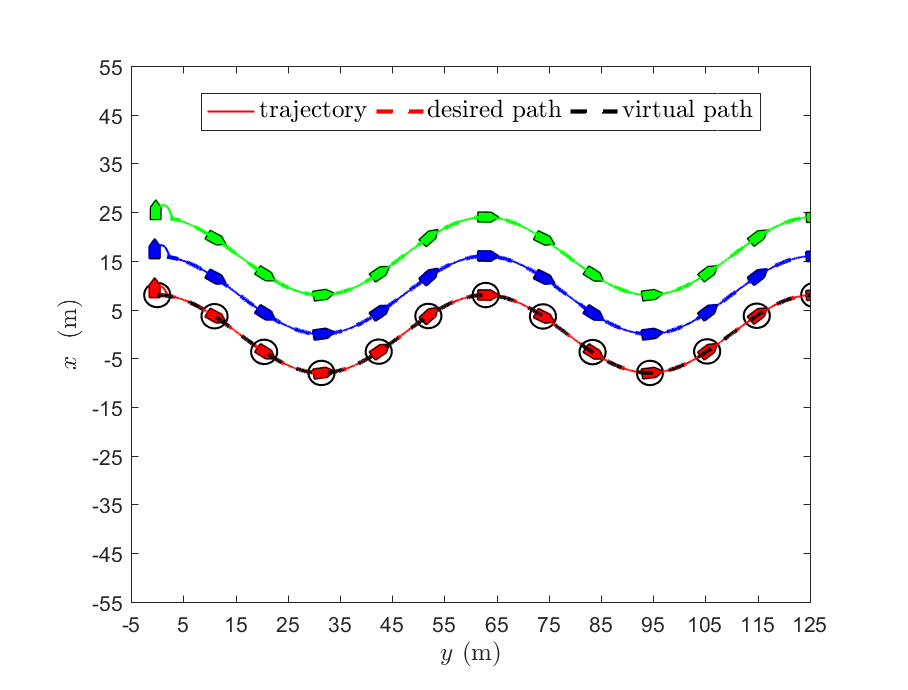
\includegraphics[width=\hsize]{map.eps}
	\caption{Coordinated path following performance.}
	\label{fig3}
\end{figure}
\begin{figure}[!htb]
	\centering
	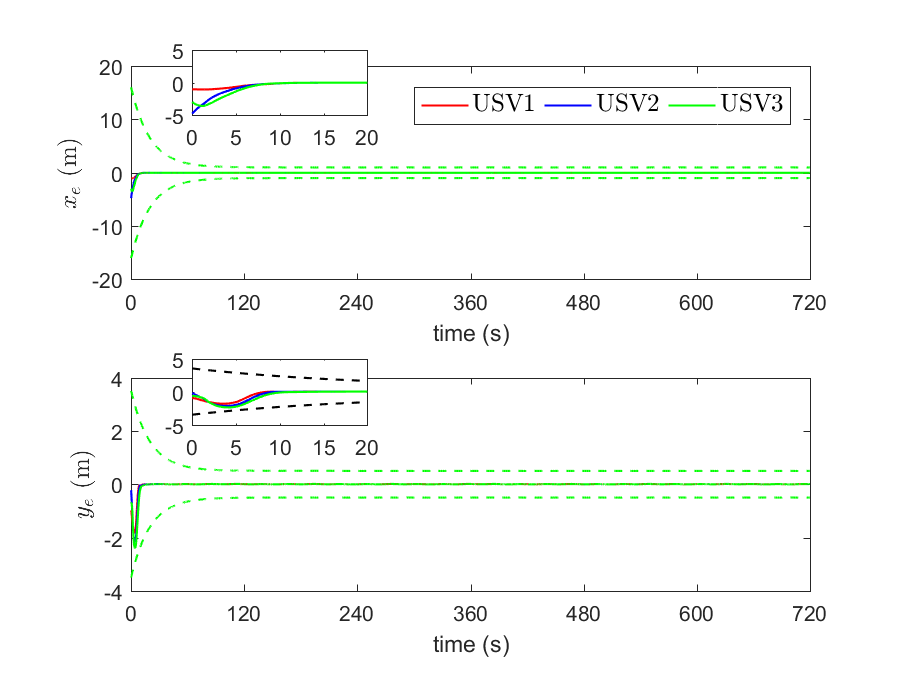
\includegraphics[width=\hsize]{CPFerror.eps}
	\caption{Path following errors.}
	\label{fig4}
\end{figure}
\begin{figure}[!htb]
	\centering
	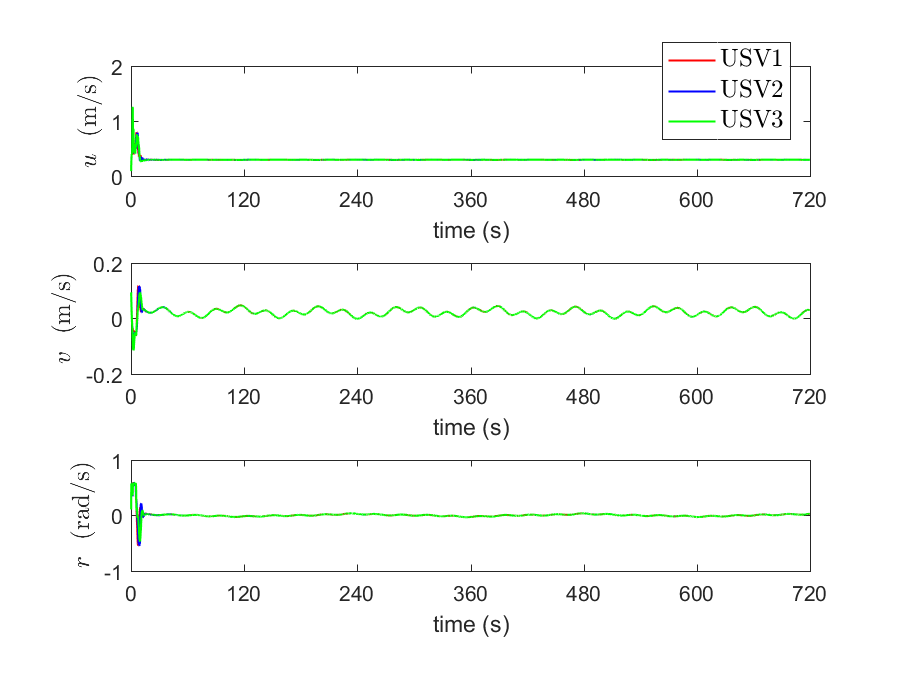
\includegraphics[width=\hsize]{velocity.eps}
	\caption{Velocities of USV.}
	\label{fig5}
\end{figure}
\begin{figure}[!htb]
	\centering
	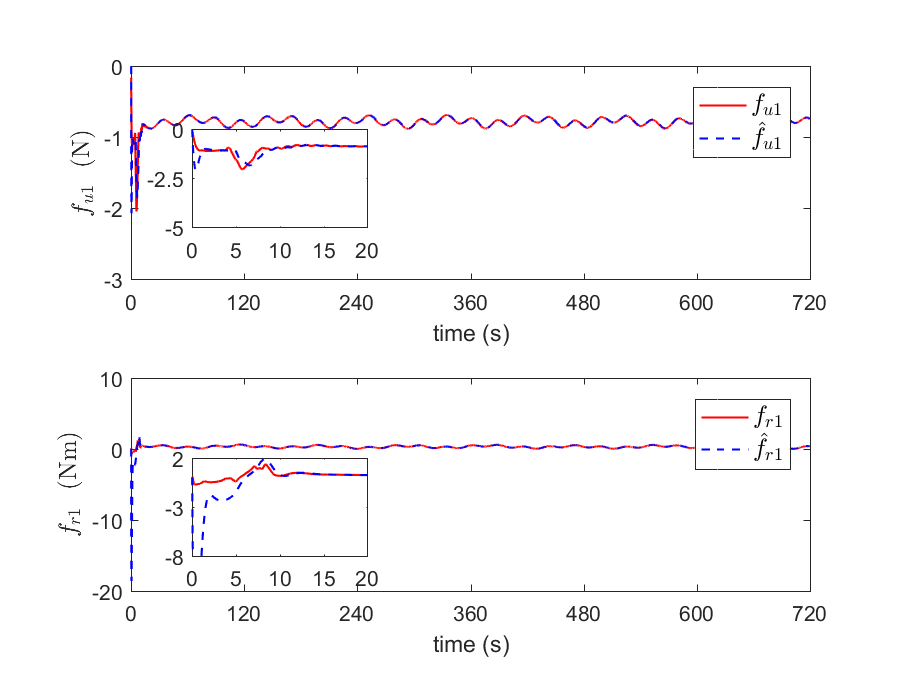
\includegraphics[width=\hsize]{RBF.eps}
	\caption{Estimations of disturbances.}
	\label{fig6}
\end{figure}
\begin{figure}[!htb]
	\centering
	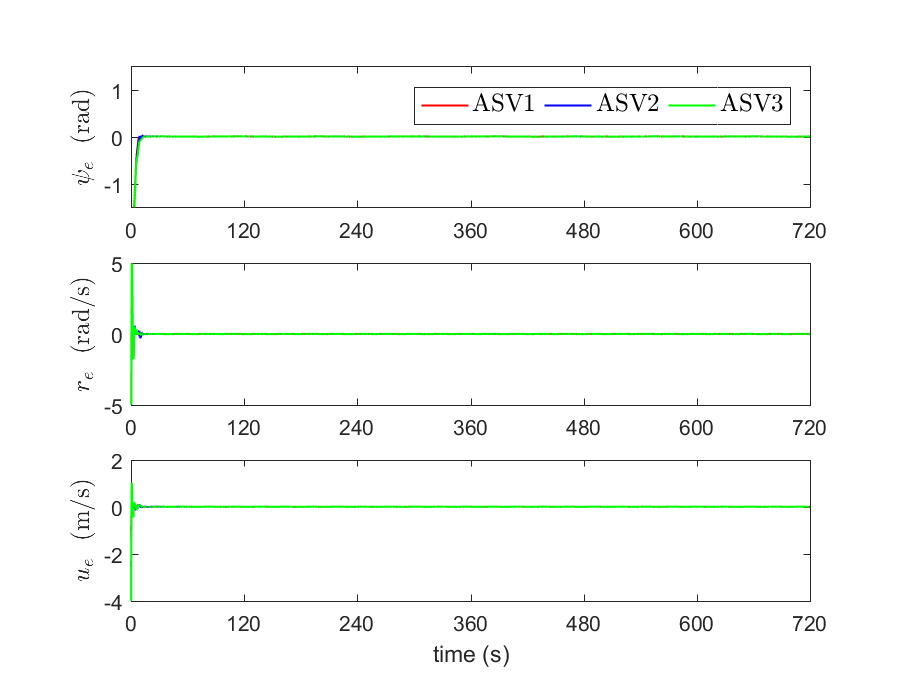
\includegraphics[width=\hsize]{trackingError.eps}
	\caption{Tracking errors of velocities.}
	\label{fig7}
\end{figure}
\begin{figure}[!htb]
	\centering
	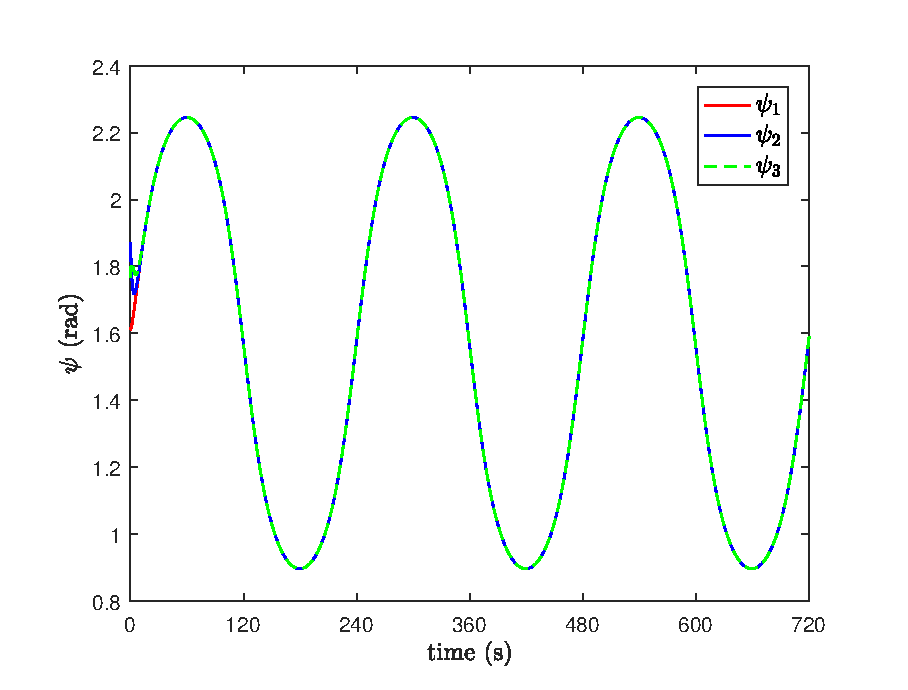
\includegraphics[width=\hsize]{headingAngle.eps}
	\caption{Heading angle of the USV.}
	\label{fig8}
\end{figure}

\begin{figure}[!htb]
	\centering
	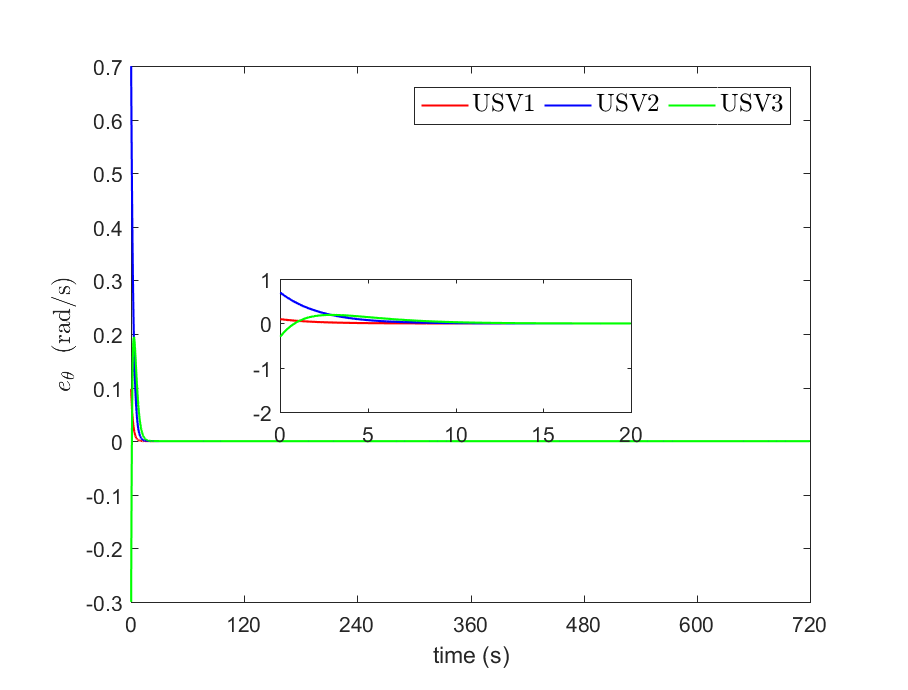
\includegraphics[width=\hsize]{coordinateError.eps}
	\caption{Coordinated errors.}
	\label{fig9}
\end{figure}

\begin{figure}[!htb]
	\centering
	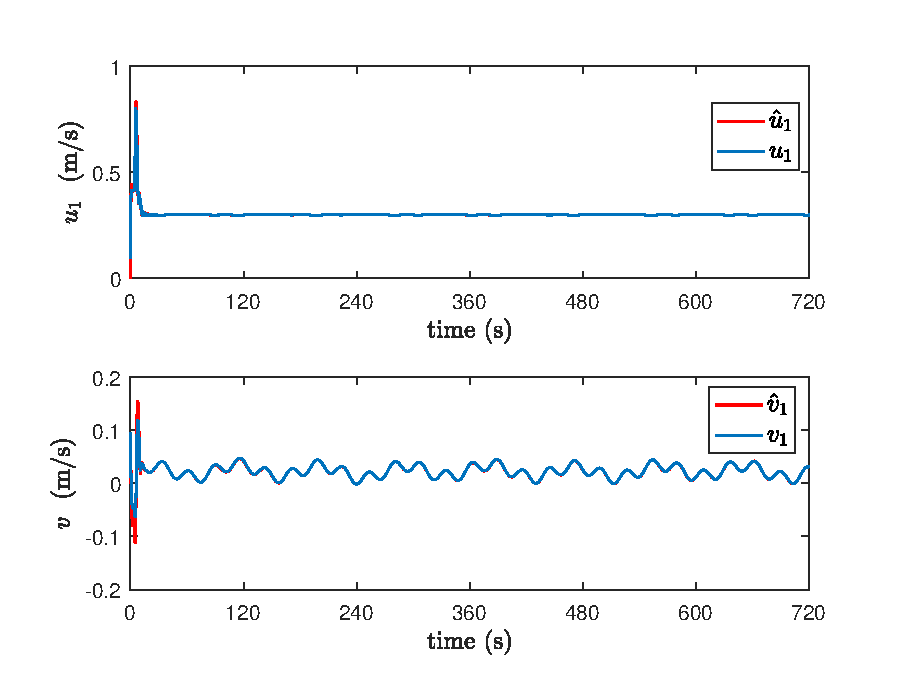
\includegraphics[width=\hsize]{NLESO.eps}
	\caption{Estimations of velocities.}
	\label{fig10}
\end{figure}

\begin{figure}[!htb]
	\centering
	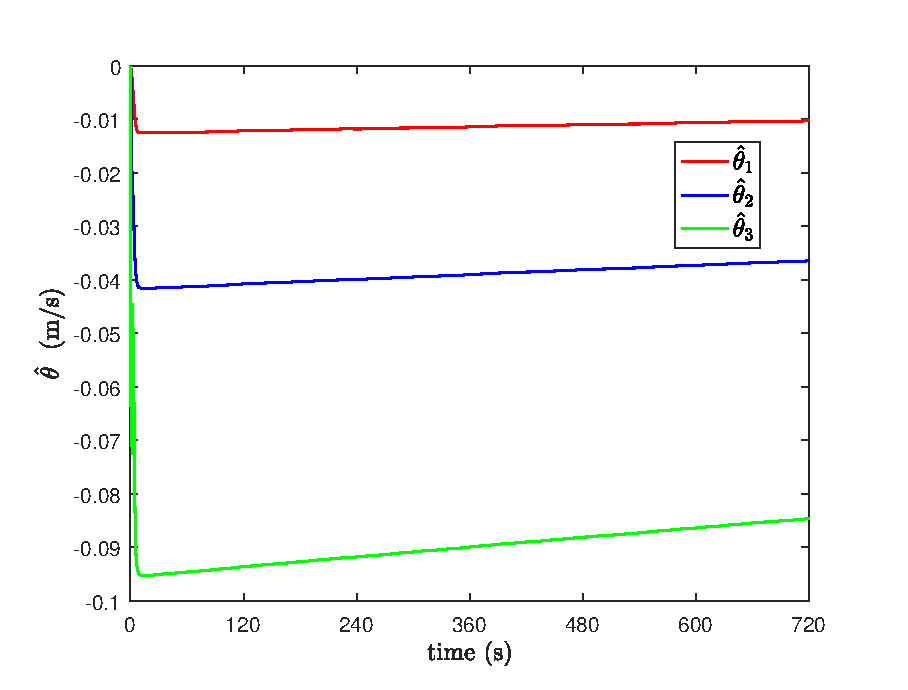
\includegraphics[width=\hsize]{AdaptiveParam.eps}
	\caption{Adaptive parameters.}
	\label{fig11}
\end{figure}



\section{Conclusion}

By combining tan-type barrier Lyapunov functions, the graph theory and the backstepping technique, this paper proposes a novel CPF guidance law. All the closed-loop errors are proved uniformly bounded by Lyapunov stability theory. In addition, the CPF erros are bounded in the prescibed boundaries. Finally, the simulations are conducted to verify the effectiveness and robustness of the proposed guidance and control system. In the future, we will consider CPF problems in which multiple USVs have the constraints of communications and collision avoidance. 

%\bibliographystyle{conferencebibtex}%if you use bibtex
%\bibliography{template}

\begin{thebibliography}{0}
	
	\bibitem{bib1} Belleter, D. J. W., Pettersen, K. Y., Path following for formations of underactuated marine vessels under influence of constant ocean currents, in \emph{Proceedings of 53rd IEEE Conference on Decision and Control}, 2014: 4521--4528. .
	
	\bibitem{bib2} Belleter, D. J. W., Braga, J., Pettersen, K. Y., Experimental Verification of a Coordinated Path-Following Strategy for Underactuated Marine Vehicles, \emph{Frontiers in Robotics and AI}, 6, 2019.
	
	\bibitem{bib3} Gu, N., Wang, D., Peng, Z. and Liu, L., Adaptive bounded neural network control for coordinated path-following of networked underactuated autonomous surface vehicles under time-varying state-dependent cyber-attack, \emph{ISA Transactions}, 104: 212--221, 2020.
	
	\bibitem{bib4} M. Lv, Z. Peng, D. Wang and Q. -L. Han, Event-Triggered Cooperative Path Following of Autonomous Surface Vehicles Over Wireless Network with Experiment Results, \emph{IEEE Trans. on Industrial Electronics}, 69(11): 11479--11489, 2022
	
	\bibitem{bib5} N. Gu, Z. Peng, D. Wang, Y. Shi and T. Wang, Anti disturbance Coordinated Path Following Control of Robotic Autonomous Surface Vehicles: Theory and Experiment, \emph{IEEE/ASME Trans. on Mechatronics}, 24(5): 2386--2396, 2019.
	
	\bibitem{bib6} Mingyu Fu, Lulu Wang, Finite-time coordinated path following control of underactuated surface vehicles based on event-triggered mechanism, \emph{Ocean Engineering}, 246, 2022.
	
	\bibitem{bib7} Peng, Z., Wang, D., Li, T. and Han, M., Output-Feedback Cooperative Formation Maneuvering of Autonomous Surface Vehicles with Connectivity Preservation and Collision Avoidance, \emph{IEEE Trans. on Cybernetics}, 50(6): 2527--2535, 2020.
	
	\bibitem{bib8} Zuo, Z., Song, J., Han and Q.-L., Coordinated Planar Path-Following Control for Multiple Nonholonomic Wheeled Mobile Robots, \emph{IEEE Trans. on Cybernetics}, 52(9): 9404--9413, 2021.
	
	\bibitem{bib9} W. Yao, H. Garcia de Marina, Z. Sun and M. Cao, Distributed coordinated path following using guiding vector fields, in \emph{Proceedings of 2021 IEEE International Conference on Robotics and Automation}, 2021: 10030--10037.
	
	\bibitem{bib10} Yao, W., Garcia de Marina, H., Sun, Z., and Cao, M., Guiding vector fields for the distributed motion coordination of mobile robots, arXiv e-prints, 2022.
	
	\bibitem{bib11} Zheng, Z., Sun, L. and Xie, L., Error-Constrained LOS Path Following of a Surface Vessel with Actuator Saturation and Faults, \emph{IEEE Trans. on Systems Man Cybernetics-Systems}, 48(10): 1794--1805, 2018.
	
	\bibitem{bib12} Zhang, Y., Wang, M., Coordinated Path Following Control of Multiple Nonholonomic Mobile Robots With Prescribed Performance, in \emph{Proceedings of 2019 Chinese Control Conference}, 2019: 5623--5628. 
	
	\bibitem{bib13} Li, C., Jiang, J., Duan, F., Liu, W., \emph{et al}., Modeling and Experimental Testing of an Unmanned Surface Vehicle with Rudderless Double Thrusters. Sensors, 19(9), 2051.
	
	\bibitem{bib14} Z. Zuo, V. Cichella, M. Xu, and N. Hovakimyan, Three-dimensional coordinated path-following control for second-order multi-agent networks, \emph{J. Franklin Inst.}, 352: 3858--3872, 2015.
	
	\bibitem{bib15} H. Zhang, F. L. Lewis, Adaptive cooperative tracking control of higher-order nonlinear systems with unknown dynamics, Automatica, 48(7): 1432--1439, 2012.
	
\end{thebibliography}


\end{document}




